\chapter[Projeto Estrutural]{Projeto Estrutural}

Nesta seção serão apresentados os avanços realizados com relação a parte que concerne ao grupo de estrutura do projeto. Serão descritos de forma sucinta os processos de fabricação envolvidos em cada subsistema do laboratório, além de todas as outras adaptações necessárias para o funcionamento do motor que será utilizado nos ensaios.

\section{Motor}

\subsection{Berço do motor}

Para que o motor fosse acoplado aos coxins do dinamômetro mostrou-se necessária a fabricação de um berço, de forma que o motor pudesse ser fixado aos coxins estando alinhado com o eixo do dinamômetro. 

Para a construção do berço do motor, visto na Figura \ref{fig:bercomotor} foi utilizado uma barra com perfil em L e espessura de 3mm com o intuito de suportar o peso e vibração causados pelo motor em funcionamento.

\begin{figure}[h!]
	\centering
	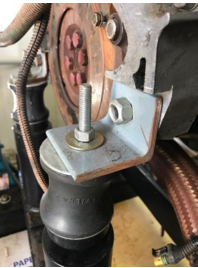
\includegraphics[keepaspectratio=true,scale= 0.8]{figuras/berco-motor.png}
	\caption{Berço do Motor Conectado.}
	\label{fig:bercomotor}
\end{figure}

Para o acoplamento tanto para o motor quanto para os coxins foram realizados furos com a furadeira com diâmetros de 10mm para os coxins e 12mm para o motor. Conforme mostrado na Figura \ref{fig:bercomotor}, uma parte da caixa seca necessitou de usinagem para facilitar o encaixe do berço.

\subsection{Parte Elétrica do Motor}

Em relação a parte elétrica do motor foi retirado todo o chicote do veículo para que fosse instalado na bancada. Ao tentar instalar pela primeira vez não foi possível ligar o motor, pois existiam alguns curtos circuitos no chicote, isto foi solucionado verificando a continuidade ao longo de todo o chicote. Porém ao tentar executar várias partidas no motor a central eletrônica (ECU) do motor entrou em modo de segurança, travando a alimentação dos bicos injetores e da bobina do motor. A solução eliminar os erros de bloqueio da ECU e também foi feito a decodificação da mesma através de um scanner. A decodificação foi feita para simplificar o chicote, pois ela elimina o uso do comutador de ignição, que é um sistema de segurança da Fiat, chamado de Fiat Code. Após a decodificação da ECU o chicote foi simplificado apenas ao molho da chave, onde se tem a ligação do motor e um fio de pós chave, onde alimenta todo o sistema da ECU ao girar a chave em seu primeiro estágio.

Foi decidido ligar o ventilador do sistema de arrefecimento no fio de pós chave, pois em um veículo o fluxo de ar gerado ao movimentar ajuda na transferência de calor do radiador. No nosso caso, como o motor está em uma bancada, o ventilador estará ligado continuamente desde o momento em que ligar a chave. 

Para bomba de combustível, esta foi alimentada diretamente pela ECU e o aterramento foi feito juntamente com o bloco do motor. 


\subsection{Parte Elétrica do Motor}

Para que a unidade de controle eletrônico do motor não ficasse pendurada, um suporte foi fabricado e acoplado ao motor. O suporte feito com uma placa de aço de 1mm de espessura, garantiu que a ECU não ficasse em contato direto com o bloco do motor. A Figura \hyperref[fig:ecu]{2a} apresenta o suporte sem a ECU enquanto a Figura \hyperref[fig:ecu]{2b} apresenta com a ECU acoplada.

\begin{figure}[h!]
\begin{center}
	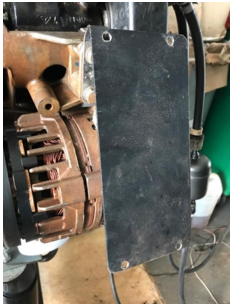
\includegraphics[height=5cm]{figuras/suporte-ecu.png} \quad
	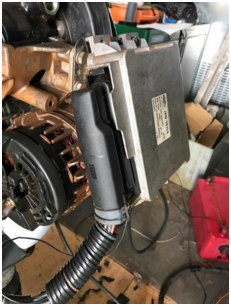
\includegraphics[height=5cm]{figuras/ecu-acoplada.png}
	\caption{a) Suporte da ECU e b) ECU Acoplada ao Suporte.}
 	\label{fig:ecu}
\end{center}
\end{figure}

Para a construção do suporte foi necessário realizar quatro furos de 6 mm para a fixação da ECU. Além disso foi, outros dois furos de 10 mm de diâmetro foram realizados para fixação do suporte no motor e do aterramento da ECU.

\section{Arrefecimento}

O sistema de arrefecimento do motor é composto pelo radiador, localizado na parte de fora do laboratório de testes. Optou-se por colocar o radiador do lado de fora do container pois ao se realizar ensaios a temperatura interna do laboratório se eleva, podendo afetar o rendimento do radiador. Além disso, para evitar o calor absorvido pelas paredes do container, optou-se por colocar o radiador de forma perpendicular, conforme demonstrado nas Figura \hyperref[fig:vistaradiador]{3a} e Figura \hyperref[fig:vistaradiador]{3b}.

\begin{figure}[h!]
\begin{center}
	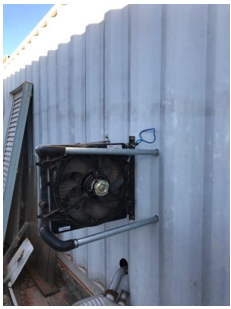
\includegraphics[height=5cm]{figuras/vista-traseira-radiador.png} \quad
	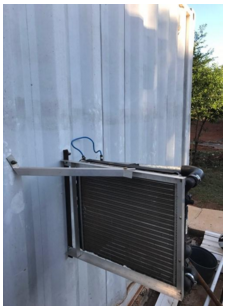
\includegraphics[height=5cm]{figuras/vista-dianteira-radiador.png}
	\caption{a) Vista Traseira do Radiador e b) Vista Dianteira do Radiador.}
 	\label{fig:vistaradiador}
\end{center}
\end{figure}

Conforme apresentado na Figura \hyperref[fig:vistaradiador]{3b}, uma estrutura de 500x430mm em alumínio foi fabricada, além de um braço diagonal para evitar o deslocamento longitudinal excessivo do radiador. Para aguentar a tensão cisalhante causada pelo peso do radiador, optou-se que a fixação da moldura contendo o radiador fosse presa com parafusos com 12mm de diâmetro.

Para a instalação do sistema de arrefecimento também foi necessária a adaptação do sistema de mangueiras. Uma vez que não possuíam comprimento suficiente para chegar ao lado de fora do container, foi necessário adaptá-las com novas mangueiras de 33mm de diâmetro interno e canos rígidos também com o mesmo diâmetro. Tendo em vista que as temperaturas do fluido de arrefecimento podem chegar a até 100ºC, foi necessário se realizar um estudo sobre os materiais que poderiam ser utilizados para realizar a circulação da água. Durante a pesquisa, materiais como PVC e CPVC se mostraram inviáveis devido a seus limites de temperatura de operação. Já a opção do cano de cobre se mostrou inviável devido a seu custo elevado e necessidade de solda para cada conexão. Tendo isto em vista, optou-se pelo uso de mangueiras de borracha com 3mm de espessura para a parte interna do container (Figura \ref{fig:caixaestabilizadora}) ligadas com auxílio de abraçadeiras a tubos de aço revenido (Figura \hyperref[fig:vistaradiador]{3a}) com 2mm de espessura na parte externa do container


\section{Admissão de Ar}

Para o sistema de admissão de ar do motor, julgou-se necessário a adição de uma caixa estabilizadora de ar. Esta caixa tem a função de minimizar o efeito de pulsação causado pelo motor fazendo com que o fluxo de ar para o motor seja mais constante. Isso facilita a obtenção de dados com relação a vazão mássica de ar no motor. A caixa estabilizadora, diferente do projeto apresentado previamente, foi alocada na parte superior do container. Para sua fixação foram utilizados furos de 8mm de diâmetro além de uma manta de borracha para evitar infiltração de água para dentro do container em épocas chuvosas. A Figura \ref{fig:caixaestabilizadora} apresenta a caixa estabilizadora utilizada no projeto.

\begin{figure}[h!]
	\centering
	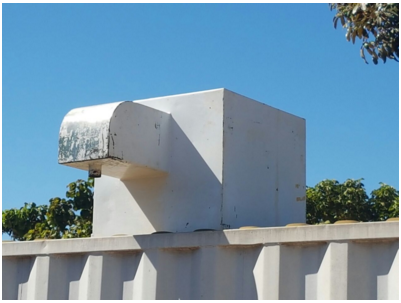
\includegraphics[keepaspectratio=true,scale= 0.6]{figuras/caixa-estabilizadora.png}
	\caption{Caixa Estabilizadora sobre o Container.}
	\label{fig:caixaestabilizadora}
\end{figure}

Para fazer a ligação da caixa estabilizadora com o coletor de admissão do motor será utilizada uma mangueira de 2m de comprimento e 50mm de diâmetro interno sem a necessidade de apresentar uma espessura ou material específico uma vez que o ar entra em temperaturas ambientes no motor.

\vfill

\section{Sistema de Exaustão}

O processo de exaustão do motor deve ser tratado com cautela uma vez que os gases resultantes da combustão são nocivos além de serem expulsos pelo coletor de escape a altíssimas temperaturas. Outro fator que deve ser levado em conta é o ruído causado pelo funcionamento do motor que caso não seja abafado pode chegar a até 100 dB. Portanto, para que o sistema de exaustão atendesse a todos esses pré requisitos citados anteriormente, foi necessário fabricar um sistema que fosse capaz de expulsar os gases do container sem e diminuir o ruído gerado pelo motor, utilizando um material que resista a altas temperaturas.

Aproveitando a saída do coletor de escape e o flexível que seguia depois dele, foi necessário criar um sistema que pudesse ser rosqueado à mangueira flexível que seguirá para a saída do container. Um dos lados da mangueira foi conectado ao coletor de escape do motor enquanto o outro foi conectado ao sistema escapamento e abafadores disponível.

A Figura \ref{fig:exaustao} apresenta a disposição externa do sistema de escape do motor. Pode-se perceber que o escapamento apresenta dois abafadores de som fazendo com que a percepção de ruídos seja atenuada drasticamente do lado externo do laboratório ao se realizar ensaios.

\begin{figure}[h!]
	\centering
	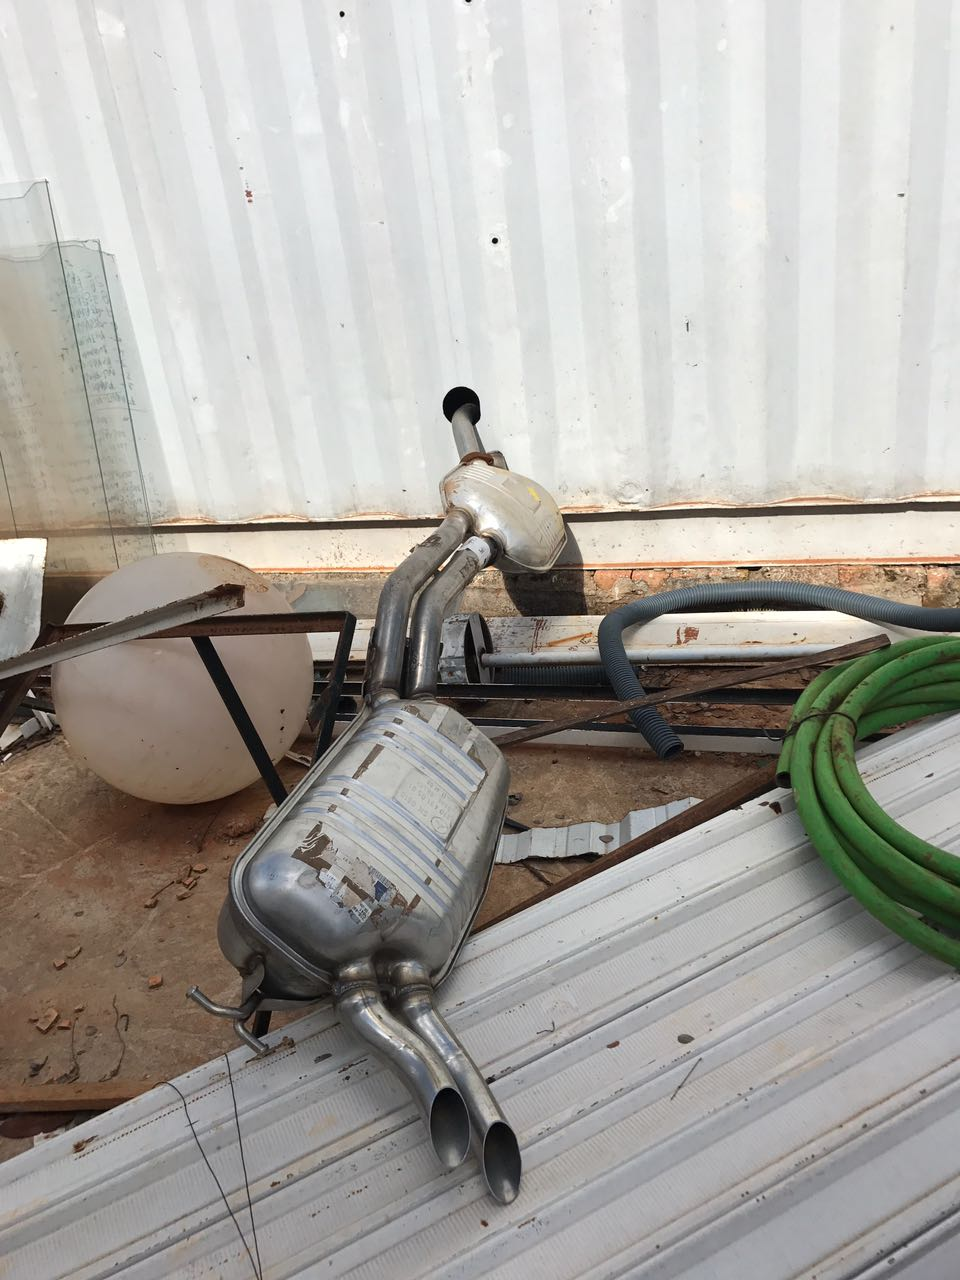
\includegraphics[keepaspectratio=true,scale= 0.2]{figuras/exautao.jpeg}
	\caption{Sistema de Exaustão.}
	\label{fig:exaustao}
\end{figure}


	
\section{Sistema de Alimentação}

A alimentação de combustível para o motor será feita com bomba de combustível, por injeção eletrônica. O tanque para armazenamento de combustível foi adaptado para fixação no laboratório e para atender aos requisitos para o cálculo de medição de consumo.

A medição de consumo é realizada a partir da variação mássica de combustível medida por uma célula de carga. A celula de carga foi acoplada ao conteiner, através de uma estrutura de fixação e o tanque é fixo a ela por correntes de aço. A figura \ref{celulaDeCarga} ilustra a célula de carga utilizada. 

\begin{figure}[h!]
	\centering
	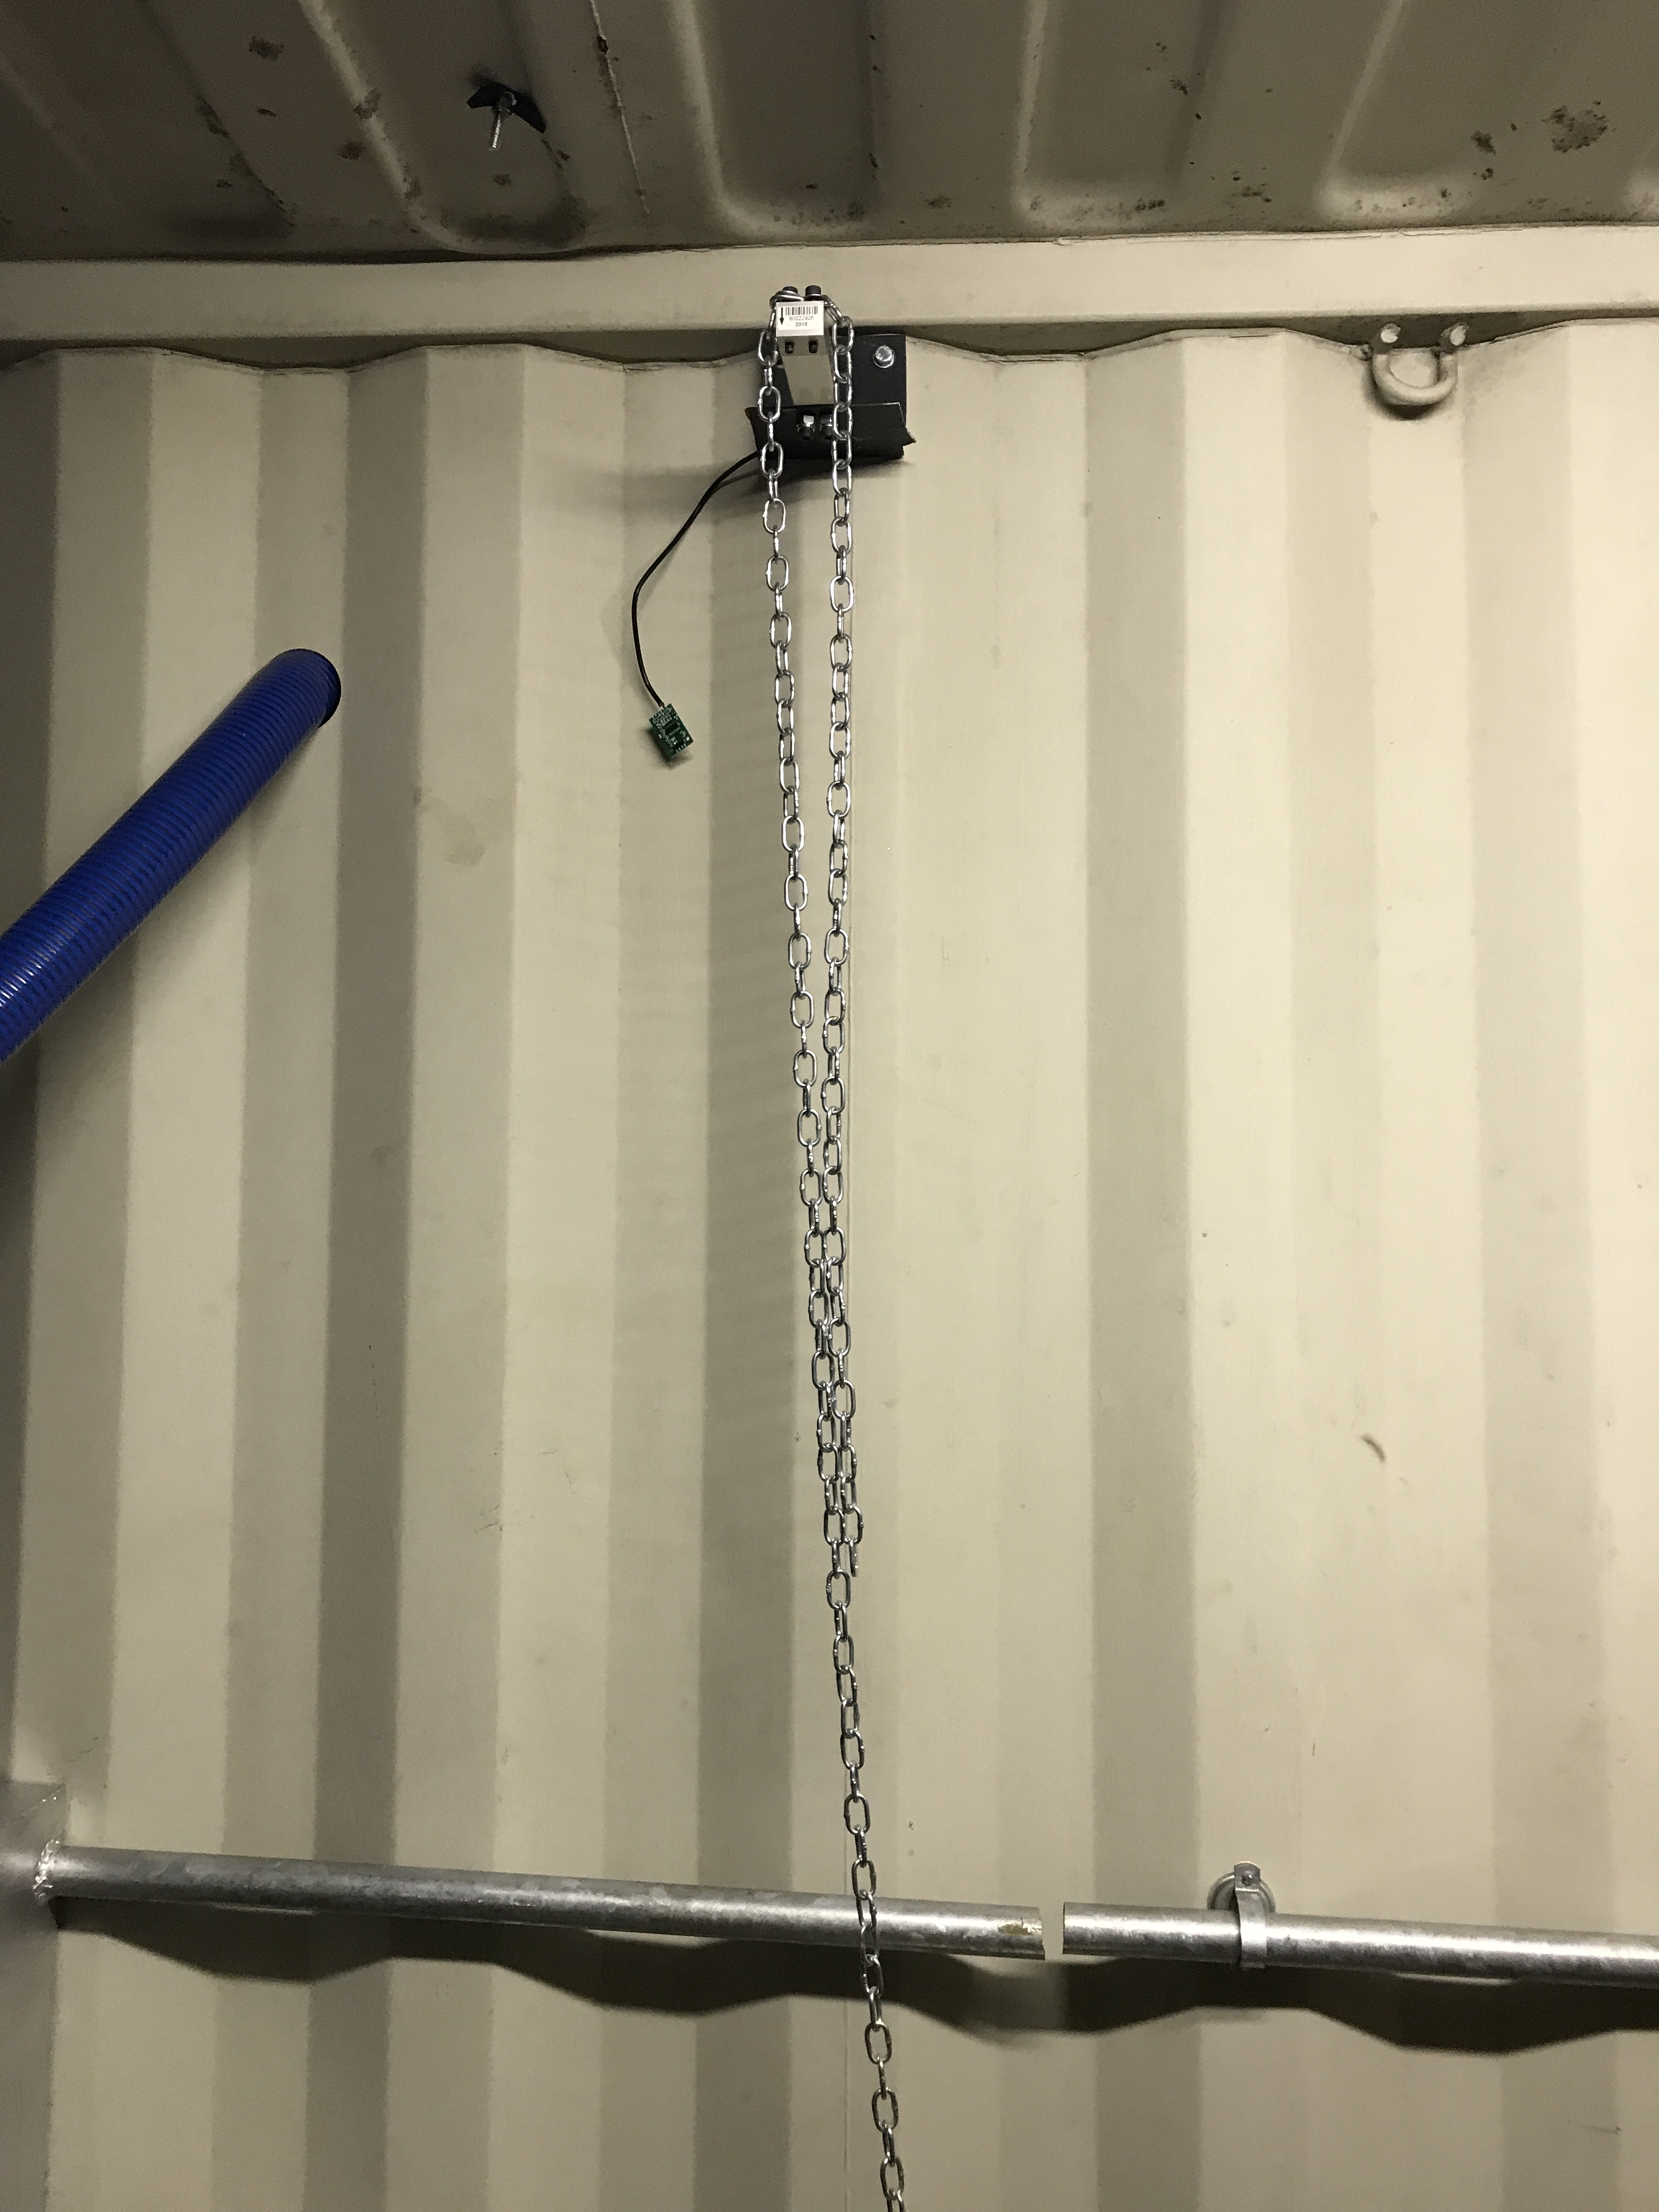
\includegraphics[keepaspectratio=true,scale= 0.07]{figuras/celulaDeCarga.JPG}
	\caption{Célula de carga.}
	\label{celulaDeCarga}
\end{figure}

\vfill

\section{Acoplamento ao Dinamômetro}

Para o acoplamento do motor ao dinamômetro foi fabricada uma flange móvel nas extremidades e feita de aço estrutural. O fator importante para concepção desta peça para o acoplamento é o torque que será aplicado a ela pelo motor. Com a conexão feita, o torque gerado pelo motor é aplicado ao dinamômetro, que será capaz de dimensionar este torque. A Figura \ref{fig:flange} apresenta a geometria da flange de acoplamento.

\begin{figure}[h!]
	\centering
	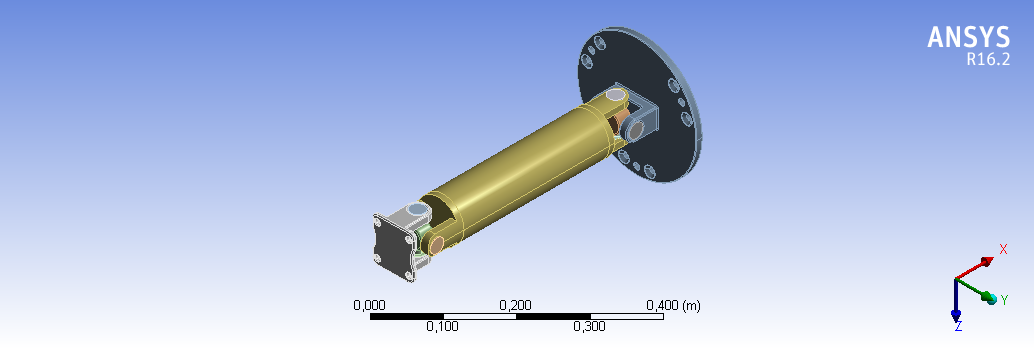
\includegraphics[keepaspectratio=true,scale= 0.35]{figuras/Geometria.png}
	\caption{Flange de Acoplamento do Motor.}
	\label{fig:flange}
\end{figure}

O critério adotado para fabricação da flange é de suportar o torque produzido pelo motor quando o dinamômetro aciona o freio. As Figuras \ref{fig:tesaoequivalente} e \ref{fig:fatorseguranca} mostram a tensão equivalente na peça quando aplicado o torque máximo e o fator de segurança, respectivamente, calculados através da simulação estrutural da peça de acoplamento.


\begin{figure}[h!]
	\centering
	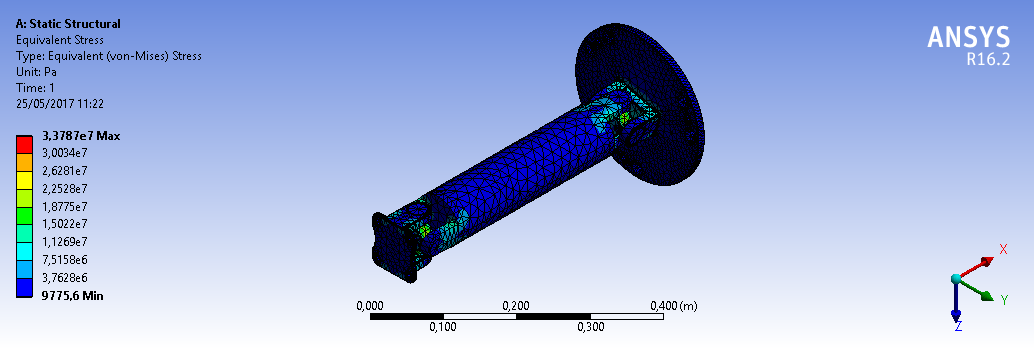
\includegraphics[keepaspectratio=true,scale= 0.35]{figuras/Tensao_Equivalente.png}
	\caption{Tensão Equivalente na Peça.}
	\label{fig:tesaoequivalente}
\end{figure}

\begin{figure}[h!]
	\centering
	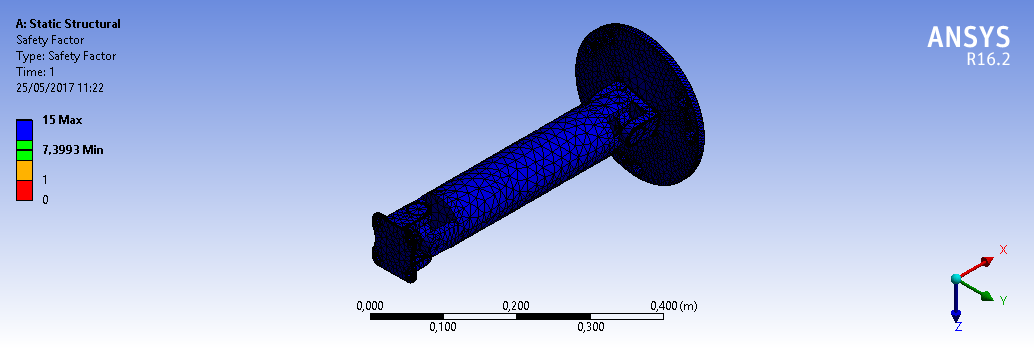
\includegraphics[keepaspectratio=true,scale= 0.33]{figuras/Fator_de_Seguranca.png}
	\caption{Fator de Segurança.}
	\label{fig:fatorseguranca}
\end{figure}

\vfill

Vale ressaltar que as simulações foram feitas considerando a extremidade de acoplamento ao dinamômetro fixa, simulando o momento de frenagem. O torque aplicado à extremidade de acoplamento ao motor foi de 88.26 N.m, valor de torque máximo para o motor em questão de acordo com  tabela FIAT.

As simulações demonstraram que a tensão máxima suportada na flange será de 38.177 MPa e o fator de segurança para a operação com o torque solicitado será de 7.4. Os resultados foram satisfatórios já que comprovam que a peça não sofrerá nenhuma falha estrutural e nem será submetida ao seu limite suportado.


\section{Projeto da Estrutura de Acoplamento do Motor}

Partindo das premissas do projeto, foi desenvolvida uma estrutura para acoplamento do motor. Ela deveria suportar o peso do propulsor na análise estática e na análise dinâmica, do tipo modal, suas frequências naturais deveriam aparecer acima de 116 Hertz, frequência de oscilação do motor a 3500 rotações por minuto.

Partindo dos pontos de apoio do motor, foi desenvolvido um modelo em CAD 3D da estrutura para análise em método dos elementos finitos em software numérico. A estrutura para as análises foi simplificada a fim de redução no custo computacional. A Figura \ref{fig:estrutura3D} apresenta o modelo descrito.

\begin{figure}[h!]
	\centering
	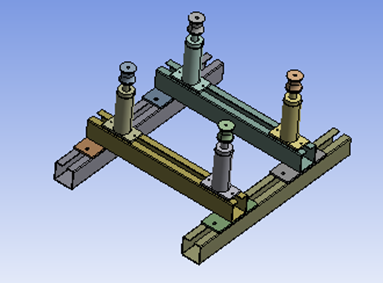
\includegraphics[keepaspectratio=true,scale= 0.8]{figuras/estrutura-3D.png}
	\caption{Modelo simplificado da estrutura em CAD 3D para análise numérica.}
	\label{fig:estrutura3D}
\end{figure}

O modelo da estrutura fornece liberdade de ajuste dos pontos de fixação do motor nos 3 eixos. Foram inseridos absorvedores de vibração nos quatro locais de conexão entre o motor e a estrutura. A Tabela \ref{tab:pontosfixacao} apresenta as distâncias máximas de mínimas que a estrutura possibilita para fixação do motor. Foi utilizado o extremo inferior da estrutura para comparação as medidas do eixo z.

\begin{figure}[h!]
	\centering
	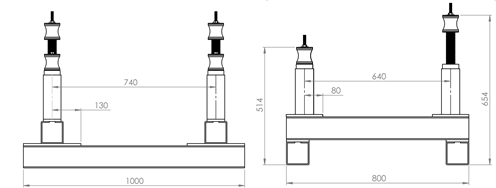
\includegraphics[keepaspectratio=true,scale= 0.8]{figuras/dimensionamento.png}
	\caption{Dimensionamento da Estrutura.}
	\label{fig:dimensionamento}
\end{figure}


\begin{table}[!h]
\centering
\caption{Liberdade para posicionamento dos pontos de fixação nos três eixos (x, y e z)}
\label{tab:pontosfixacao}
\begin{tabular}{|l|l|l|}
\hline
\multicolumn{1}{|c|}{\textbf{Eixo}}    & \multicolumn{1}{c|}{\textbf{Distância Máxima (mm)}} & \multicolumn{1}{c|}{\textbf{Distância Mínima (mm)}} \\ \hline
x        					   & 260                             & 740                \\ \hline
y       					   & 180                              & 640               \\ \hline
z             				   & 514                              & 654            \\ \hline
\end{tabular}
\end{table}


\pagebreak

Os materiais utilizados para análise numérica foram o aço carbono 1020, que possui tensão de escoamento de 210 MPa, e o polímero polietireno, com tensão de escoamento de 25 Mpa.

As análises numéricas foram realizadas na plataforma Workbench do software Ansys e foi utilizado o maior grau de refino na malha.

Nas condições de contorno da análise estática, foram inseridas a gravidade do planeta Terra, a restrição total na movimentação dos dois perfis inferiores da estrutura, cujo ficam fixos ao solo, e as forças pontuais de 350 Newtons nos quatro pontos de acoplamento com o motor. Estas condições de contorno podem ser observadas na Figura \ref{fig:analiseestatica}.

\begin{figure}[h!]
	\centering
	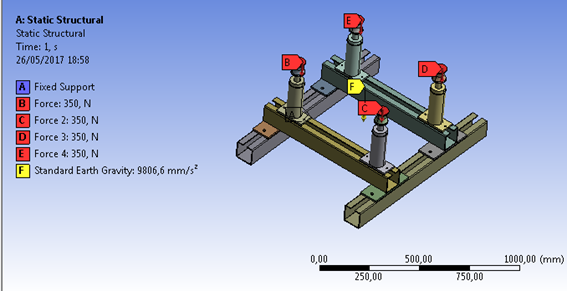
\includegraphics[keepaspectratio=true,scale= 0.8]{figuras/analise-estatica.png}
	\caption{Condições de contorno para a análise estática.}
	\label{fig:analiseestatica}
\end{figure}

Na análise modal da estrutura também foi restrita a movimentação nos locais de fixação ao solo, conforme apresentado na Figura \ref{fig:analisemodal}.

\begin{figure}[h!]
	\centering
	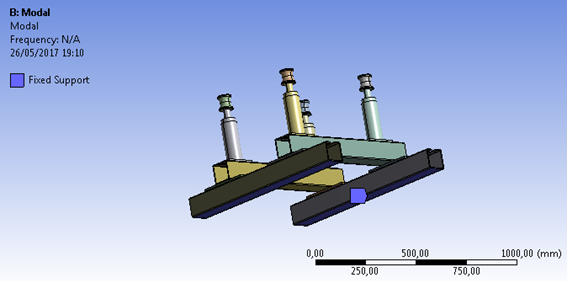
\includegraphics[keepaspectratio=true,scale= 0.8]{figuras/analise-modal.png}
	\caption{Condições de Contorno para a Análise Modal.}
	\label{fig:analisemodal}
\end{figure}


Pela análise estática, conforme resultados nas Figuras \ref{fig:deformacao}, \ref{fig:pascal} e \ref{fig:coeficienteestrutura}, a máxima tensão que a estrutura estará submetida será de XXX MPa, assim, ela estará apta a receber o peso do motor. Os locais onde estão presentes o material de menor tensão de escoamento, logo, foram onde obteve-se maior deformação da estrutura, algo já esperado, porém toda a estrutura apresenta coeficiente de segurança de, pelo menos, 15.

\begin{figure}[h!]
	\centering
	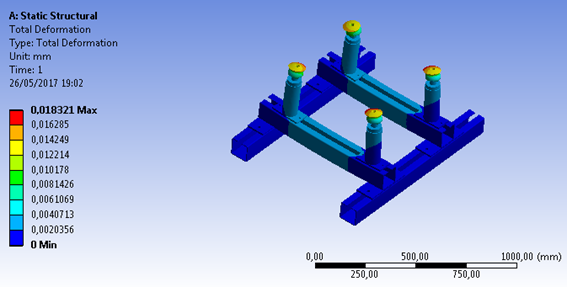
\includegraphics[keepaspectratio=true,scale= 0.8]{figuras/resultado-deformacao.png}
	\caption{Resultado de Deformação da Estrutura.}
	\label{fig:deformacao}
\end{figure}

\begin{figure}[h!]
	\centering
	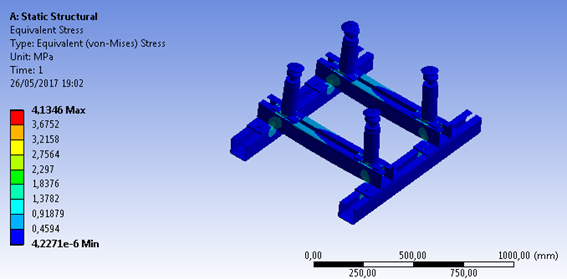
\includegraphics[keepaspectratio=true,scale= 0.8]{figuras/pascal.png}
	\caption{Respostas de tensão equivalente da estrutura em Mega Pascal.}
	\label{fig:pascal}
\end{figure}

\begin{figure}[h!]
	\centering
	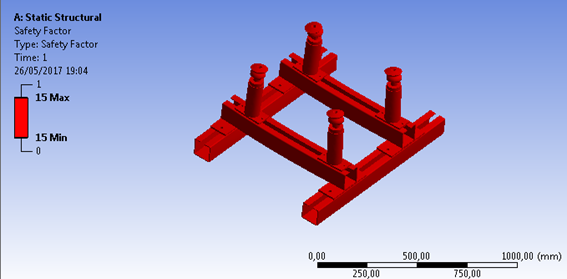
\includegraphics[keepaspectratio=true,scale= 0.8]{figuras/coeficiente-estrutura.png}
	\caption{Coeficiente de segurança da estrutura.}
	\label{fig:coeficienteestrutura}
\end{figure}

\pagebreak

 Pela análise modal, vide resultados na Tabela \ref{tab:frequencias}, a estrutura respondeu com sua primeira frequência natural em 128,32 Hertz. Logo, também houve aprovação neste quesito.


\begin{table}[!h]
\centering
\caption{Frequências naturais da estrutura.}
\label{tab:frequencias}
\begin{tabular}{|l|l|}
\hline
\multicolumn{1}{|c|}{\textbf{Modo}}    & \multicolumn{1}{c|}{\textbf{Frequência (Hertz)}} \\ \hline
1        					   & 128,32          \\ \hline
2       					   & 128,33         \\ \hline
3            				   & 138,11          \\ \hline
4        					   & 178,41          \\ \hline
5       					   & 178,57          \\ \hline
6            				   & 208,51          \\ \hline
7       					   & 288,22          \\ \hline
8            				   & 288,6          \\ \hline
9       					   & 426,53         \\ \hline
10           				   & 458,97          \\ \hline
\end{tabular}
\end{table}